% =====================================================================
%  Ingenieria de Requisitos (ISR-401) -- UTEQ
%  PRUEBA PRACTICA -- UNIDAD IV -- PARALELO B
%  Estudiante: Zambrano Moya Angelo Paul
%  Caso: Sistema de Reserva de Citas Medicas
%  Desarrollo resuelto: P1 a P7. P8, P9 y P10 se conservan sin resolver.
%  Compilacion recomendada en Overleaf: pdfLaTeX
% =====================================================================
\documentclass[11pt,a4paper,oneside]{article}

\usepackage[utf8]{inputenc}
\usepackage[T1]{fontenc}
\renewcommand{\tablename}{Tabla}
\renewcommand{\figurename}{Figura}
\usepackage[scaled=0.92]{helvet}
\usepackage{textcomp}
\usepackage[a4paper,top=2.4cm,bottom=2.3cm,left=2.5cm,right=2.3cm,headheight=15pt]{geometry}
\usepackage{amsmath,amssymb}
\usepackage{graphicx}
\usepackage{tikz}
\usetikzlibrary{positioning,shapes.multipart,shapes.geometric,arrows.meta,calc,fit}
\usepackage[table,dvipsnames]{xcolor}
\usepackage{array}
\usepackage{tabularx}
\usepackage{multirow}
\usepackage{colortbl}
\usepackage{booktabs}
\usepackage{enumitem}
\usepackage[protrusion=true,expansion=false]{microtype}
\usepackage{parskip}
\usepackage{titlesec}
\usepackage{fancyhdr}
\usepackage{caption}
\usepackage{pdflscape}
\usepackage[numbers,sort&compress]{natbib}
\usepackage[colorlinks=true,linkcolor=darkblue,citecolor=darkblue,urlcolor=midblue,
  pdftitle={Prueba Practica Unidad IV - Paralelo B - Ingenieria de Requisitos ISR-401},
  pdfauthor={Zambrano Moya Angelo Paul - UTEQ}]{hyperref}
\usepackage[most]{tcolorbox}

% Paleta institucional
\definecolor{darkblue}{HTML}{1A3A5C}
\definecolor{midblue}{HTML}{2E6DA4}
\definecolor{gold}{HTML}{C8A951}
\definecolor{lightgray}{HTML}{F2F2F2}
\definecolor{rowgray}{HTML}{EEEEEE}
\definecolor{softblue}{HTML}{EAF1F8}
\definecolor{softred}{HTML}{F7E7E7}
\definecolor{darkred}{HTML}{9C2A2A}
\definecolor{softgreen}{HTML}{E7F1E7}

% Interlineado y columnas
\linespread{1.05}
\setlength{\parskip}{5pt}
\setlength{\parindent}{0pt}
\renewcommand{\arraystretch}{1.25}
\newcolumntype{L}[1]{>{\raggedright\arraybackslash}p{#1}}
\newcolumntype{C}[1]{>{\centering\arraybackslash}p{#1}}
\newcolumntype{R}[1]{>{\raggedleft\arraybackslash}p{#1}}

% Encabezados
\titleformat{\section}{\sffamily\large\bfseries\color{darkblue}}{\thesection}{0.6em}{}
  [\vspace{-5pt}{\color{gold!85}\rule{\linewidth}{1pt}}]
\titlespacing*{\section}{0pt}{14pt}{6pt}
\titleformat{\subsection}{\sffamily\normalsize\bfseries\color{midblue}}{\thesubsection}{0.5em}{}
\titlespacing*{\subsection}{0pt}{10pt}{3pt}

\pagestyle{fancy}
\fancyhf{}
\renewcommand{\headrulewidth}{0.4pt}
\fancyhead[L]{\footnotesize\sffamily\color{darkblue}Prueba Pr\'actica\, \textbullet\, Unidad IV\, \textbullet\, Paralelo B}
\fancyhead[R]{\footnotesize\sffamily\color{darkblue}Ingenier\'ia de Requisitos\, \textbullet\, ISR-401}
\fancyfoot[C]{\footnotesize\sffamily\color{darkblue}\thepage}

\captionsetup{font=small,labelfont={bf,sf,color=darkblue},labelsep=period,skip=5pt}

% Cajas
\newtcolorbox{concepto}[1]{colback=softblue,colframe=darkblue,boxrule=0.6pt,arc=2.5pt,
  left=7pt,right=7pt,top=5pt,bottom=5pt,fonttitle=\bfseries\sffamily\color{white},
  coltitle=white,colbacktitle=darkblue,title={#1},breakable}
\newtcolorbox{piso}[1]{colback=softred,colframe=darkred,boxrule=1pt,arc=2.5pt,
  left=7pt,right=7pt,top=5pt,bottom=5pt,fonttitle=\bfseries\sffamily\color{white},
  coltitle=white,colbacktitle=darkred,title={#1},breakable}
\newtcolorbox{tarea}[1]{colback=white,colframe=midblue,boxrule=0.7pt,arc=2pt,
  left=7pt,right=7pt,top=5pt,bottom=5pt,fonttitle=\bfseries\sffamily\color{white},
  coltitle=white,colbacktitle=midblue,title={#1},breakable}
\newtcolorbox{reqbox}[1]{colback=white,colframe=midblue,boxrule=0.7pt,arc=2pt,
  left=7pt,right=7pt,top=5pt,bottom=5pt,fonttitle=\bfseries\sffamily\color{white},
  coltitle=white,colbacktitle=midblue,title={#1},breakable}

\newcommand{\hd}[1]{\cellcolor{darkblue}\textbf{\textcolor{white}{\small\sffamily #1}}}
\newcommand{\hm}[1]{\cellcolor{midblue}\textbf{\textcolor{white}{\small\sffamily #1}}}
\newcommand{\hg}[1]{\cellcolor{lightgray}\textbf{\color{darkblue}\small\sffamily #1}}

% Estilos TikZ comunes
\tikzset{
  activity/.style={draw=black,rounded corners=3pt,minimum width=3.2cm,minimum height=0.8cm,align=center,font=\scriptsize,fill=white},
  decision/.style={diamond,draw=black,aspect=2.0,inner sep=1.2pt,align=center,font=\scriptsize,fill=white},
  state/.style={draw=black,rounded corners=4pt,minimum width=3.2cm,minimum height=1.1cm,align=center,font=\small\bfseries,fill=white},
  flow/.style={-{Stealth[length=2.2mm]},line width=0.75pt,draw=black},
  assoc/.style={line width=0.75pt,draw=black}
}

\begin{document}
\sffamily

% =====================================================================
% CARATULA
% =====================================================================
\thispagestyle{empty}
\begin{center}
  {\Large\bfseries\color{darkblue} UNIVERSIDAD T\'ECNICA ESTATAL DE QUEVEDO}\\[2pt]
  {\normalsize\color{midblue} Facultad de Ciencias de la Ingenier\'ia \textbullet\ Carrera de Ingenier\'ia de Software}\\[6pt]
  {\color{gold}\rule{0.9\linewidth}{1.2pt}}\\[6pt]
  {\large\bfseries\color{darkblue} PRUEBA PR\'ACTICA --- UNIDAD IV \textbullet\ PARALELO B}\\[2pt]
  {\normalsize\color{darkblue} Validaci\'on, Gesti\'on, Herramientas y Est\'andares de Requisitos}\\[2pt]
  {\small\color{black} Asignatura: Ingenier\'ia de Requisitos (ISR-401) \quad\textbullet\quad Docente: Ing. Gleiston Guerrero, Mg.}
\end{center}

\vspace{2pt}
\begin{center}\small
\begin{tabularx}{\linewidth}{@{}L{2.6cm} X L{2.6cm} X@{}}
  \hg{Estudiante} & Zambrano Moya Angelo Paul & \hg{Fecha} & 13 de agosto de 2026 \\
  \hg{Modalidad} & Individual, en clase & \hg{Duraci\'on} & 120 minutos \\
  \hg{Caso} & Sistema de Reserva de Citas M\'edicas & \hg{Ponderaci\'on} & 100 puntos (30 + 70) \\
\end{tabularx}
\end{center}

\vspace{4pt}
\begin{center}
{\small\bfseries Repositorio: \url{https://github.com/AngeloP2114/Evaluacion_Unidad_IV_Practica}}
\end{center}

\vspace{3pt}
\begin{center}
{\small\bfseries Captura del resumen del cuestionario}\\[3pt]
\includegraphics[width=0.98\linewidth,height=3.0cm,keepaspectratio]{resumen_cuestionario_SGA.png}\\[6pt]
{\small\bfseries Captura de la evaluaci\'on / revisi\'on del intento}\\[3pt]
\includegraphics[width=0.58\linewidth,height=8.0cm,keepaspectratio]{revision_intento_SGA.png}
\end{center}
\clearpage

% Resultado de aprendizaje
\begin{concepto}{Resultado de aprendizaje evaluado}
El estudiante \textbf{construye y valida} los modelos de an\'alisis (datos, funci\'on y comportamiento) de un sistema, \textbf{especifica y gestiona} sus requisitos aplicando est\'andares (\textit{ISO/IEC/IEEE} 29148:2018 e \textit{ISO/IEC} 25010:2023) y \textbf{demuestra trazabilidad, control de cambios y gesti\'on de configuraci\'on} sobre un repositorio reproducible. Esta prueba eval\'ua \emph{desempe\~no pr\'actico}: no contiene preguntas te\'oricas; se califica lo que el estudiante \emph{produce}.
\end{concepto}

% =====================================================================
\section{Instrucciones generales y entregables}

La prueba se desarrolla de forma individual durante la sesi\'on. Todo el trabajo se versiona en un \textbf{repositorio Git p\'ublico} (GitHub o GitLab) creado por el estudiante. El entregable se redacta en \textbf{LaTeX} y se compila a \textbf{PDF} dentro del propio repositorio. Al finalizar, el estudiante sube al LMS (SGA) un \textbf{PDF con car\'atula} que contiene, \textbf{en una sola l\'inea}, la \textbf{URL} del repositorio.

\begin{enumerate}[leftmargin=1.4em,itemsep=1pt,topsep=2pt]
  \item \textbf{Repositorio} con: archivo principal \texttt{.tex}, archivo \texttt{referencias.bib} (si aplica), figuras, \texttt{PDF} compilado y \texttt{README.md}.
  \item \textbf{README.md} con las instrucciones exactas de compilaci\'on: compilador (\texttt{pdflatex}), orden de comandos, archivo principal y dependencias.
  \item \textbf{Car\'atula del PDF} con datos de identificaci\'on y la URL del repositorio en una sola l\'inea, m\'as la \textbf{captura del resumen} y la \textbf{captura de la evaluaci\'on} del cuestionario rendido en el SGA.
  \item Los modelos (clases, actividades, m\'aquina de estados) pueden dibujarse en \textbf{TikZ}, en una herramienta CASE (p.\,ej. Enterprise Architect / Sparx EA) o a mano y adjuntarse como imagen legible.
\end{enumerate}

\begin{piso}{Criterios de piso --- su incumplimiento implica calificaci\'on CERO (0) en toda la prueba}
\textbf{1. Evidencia del repositorio.} El estudiante debe subir al LMS (SGA) un documento \textbf{PDF con car\'atula} (datos de identificaci\'on) que muestre claramente, \textbf{en una sola l\'inea}, la \textbf{URL del repositorio} donde se encuentra el trabajo desarrollado. Si la URL est\'a rota, el repositorio no es accesible, o no se cumple esta directriz, la calificaci\'on es \textbf{CERO}.\\[3pt]
\textbf{2. Reproducibilidad del PDF.} Si el PDF \textbf{no se genera} correctamente a partir del LaTeX mediante \textbf{clonaci\'on del repositorio y compilaci\'on} del archivo \texttt{.tex}, la calificaci\'on es \textbf{CERO}. Las instrucciones de compilaci\'on (compilador, orden de comandos, archivo principal, dependencias) deben estar documentadas en el archivo \texttt{README.md} del repositorio.
\end{piso}

% =====================================================================
\section{Caso pr\'actico: Sistema de Reserva de Citas M\'edicas}

Una cl\'inica requiere un m\'odulo para gestionar las reservas de citas de sus pacientes. Un \textbf{Paciente} (identificado por c\'edula, nombre y correo) puede solicitar cero o m\'as \textbf{Citas}. Cada \textbf{Cita} (identificador, fecha-hora y estado) corresponde a un \textbf{M\'edico} (c\'odigo, nombre, especialidad) sobre un \textbf{Cupo} de su agenda (fecha-hora, disponibilidad). Al agendar una cita, el sistema verifica la disponibilidad de \textbf{cupo} en la agenda del m\'edico: si hay cupo, \emph{confirma} la cita; si no, \emph{notifica la no disponibilidad} y propone otro horario. Una cita confirmada puede \emph{atenderse}, o bien \emph{cancelarse} mientras no haya sido atendida; si el paciente no se presenta, la cita se marca como \emph{no asistida}. El sistema debe registrar la cita con rapidez y proteger los datos personales del paciente.

Sobre este caso, el estudiante desarrolla las diez actividades pr\'acticas siguientes. Todas las actividades usan el \emph{mismo} dominio, de modo que los modelos deben ser mutuamente consistentes.

% =====================================================================
\section{Actividades pr\'acticas (desarrollo --- 70 puntos)}

% ---------------------------------------------------------------------
% P1
% ---------------------------------------------------------------------
\begin{tarea}{P1. Modelo de datos --- Diagrama de clases UML \hfill (8 pts)}
Construya el \textbf{diagrama de clases UML} del dominio con al menos las clases \textsf{Paciente}, \textsf{Cita}, \textsf{M\'edico} y \textsf{Cupo} (agenda). Cada clase debe incluir sus \textbf{atributos} con tipo, al menos una \textbf{operaci\'on} pertinente y las \textbf{multiplicidades} en los extremos de cada asociaci\'on. Subraye o marque los identificadores.
\end{tarea}

\subsection*{Respuesta P1}
\begin{center}
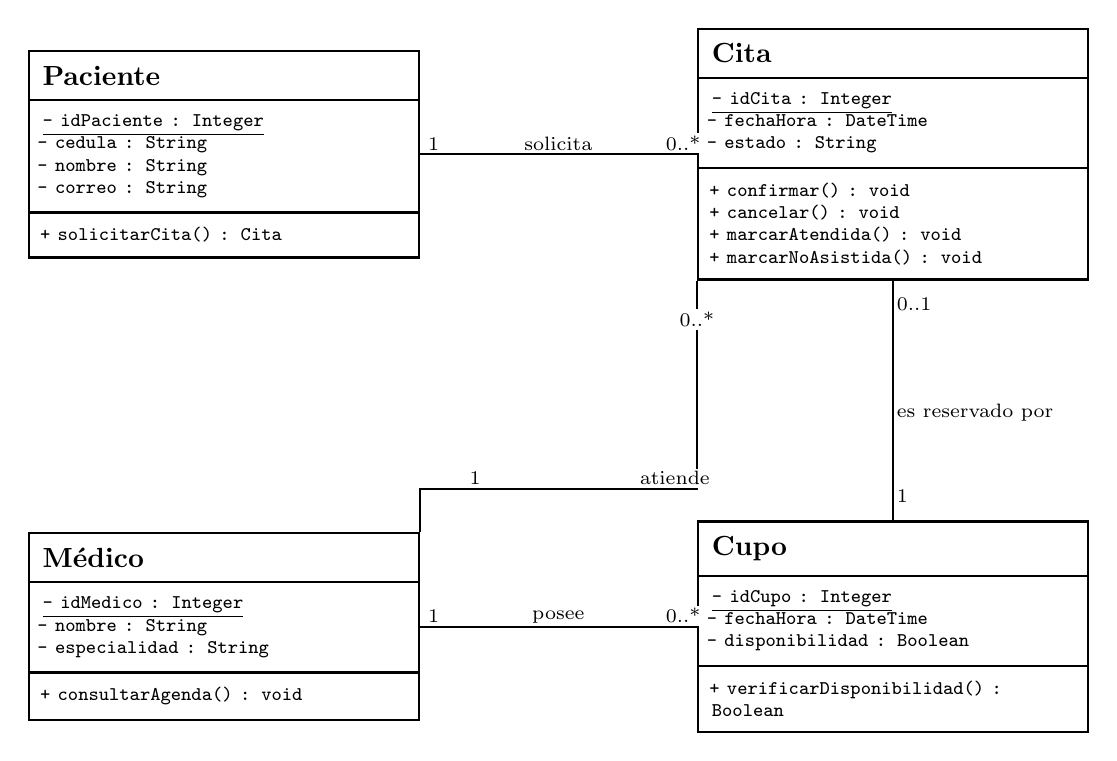
\begin{tikzpicture}[
  umlclass/.style={rectangle split,rectangle split parts=3,rectangle split part align={center,left,left},
    draw=black,line width=0.8pt,text width=4.6cm,align=left,inner sep=5pt,font=\scriptsize},
  mult/.style={font=\scriptsize,fill=white,inner sep=1pt},
  role/.style={font=\scriptsize,fill=white,inner sep=1pt}
]
\node[umlclass] (Paciente) at (-4.25,3.0) {
  {\normalsize\bfseries Paciente}
  \nodepart{second}
  \underline{\texttt{- idPaciente : Integer}}\\
  \texttt{- cedula : String}\\
  \texttt{- nombre : String}\\
  \texttt{- correo : String}
  \nodepart{third}
  \texttt{+ solicitarCita() : Cita}
};

\node[umlclass] (Cita) at (4.25,3.0) {
  {\normalsize\bfseries Cita}
  \nodepart{second}
  \underline{\texttt{- idCita : Integer}}\\
  \texttt{- fechaHora : DateTime}\\
  \texttt{- estado : String}
  \nodepart{third}
  \texttt{+ confirmar() : void}\\
  \texttt{+ cancelar() : void}\\
  \texttt{+ marcarAtendida() : void}\\
  \texttt{+ marcarNoAsistida() : void}
};

\node[umlclass] (Medico) at (-4.25,-3.0) {
  {\normalsize\bfseries M\'edico}
  \nodepart{second}
  \underline{\texttt{- idMedico : Integer}}\\
  \texttt{- nombre : String}\\
  \texttt{- especialidad : String}
  \nodepart{third}
  \texttt{+ consultarAgenda() : void}
};

\node[umlclass] (Cupo) at (4.25,-3.0) {
  {\normalsize\bfseries Cupo}
  \nodepart{second}
  \underline{\texttt{- idCupo : Integer}}\\
  \texttt{- fechaHora : DateTime}\\
  \texttt{- disponibilidad : Boolean}
  \nodepart{third}
  \texttt{+ verificarDisponibilidad() : Boolean}
};

\draw[assoc] (Paciente.east) -- node[role,above,pos=.5]{solicita}
  node[mult,above,pos=.05]{1} node[mult,above,pos=.95]{0..*} (Cita.west);
\draw[assoc] (Medico.east) -- node[role,above,pos=.5]{posee}
  node[mult,above,pos=.05]{1} node[mult,above,pos=.95]{0..*} (Cupo.west);
\draw[assoc] (Medico.north east) -- ++(0,0.55) -| node[role,above,pos=.46]{atiende}
  node[mult,above,pos=.10]{1} node[mult,above,pos=.88]{0..*} (Cita.south west);
\draw[assoc] (Cita.south) -- node[role,right,pos=.55]{es reservado por}
  node[mult,right,pos=.10]{0..1} node[mult,right,pos=.90]{1} (Cupo.north);
\end{tikzpicture}
\captionof{figure}{Diagrama de clases UML del Sistema de Reserva de Citas M\'edicas. Los identificadores se encuentran subrayados.}
\end{center}

% ---------------------------------------------------------------------
% P2
% ---------------------------------------------------------------------
\begin{tarea}{P2. Modelo funcional --- Diagrama de actividades UML \hfill (8 pts)}
Modele el proceso \textbf{``Agendar cita''} con un \textbf{diagrama de actividades UML} que incluya: nodo inicial, al menos una \textbf{decisi\'on} (\textsf{\textquestiondown cupo disponible?}), los dos caminos alternativos (\emph{confirmar} / \emph{notificar no disponibilidad}), su convergencia y el nodo final. Use carriles de responsabilidad si distingue actores.
\end{tarea}

\subsection*{Respuesta P2}
\begin{center}
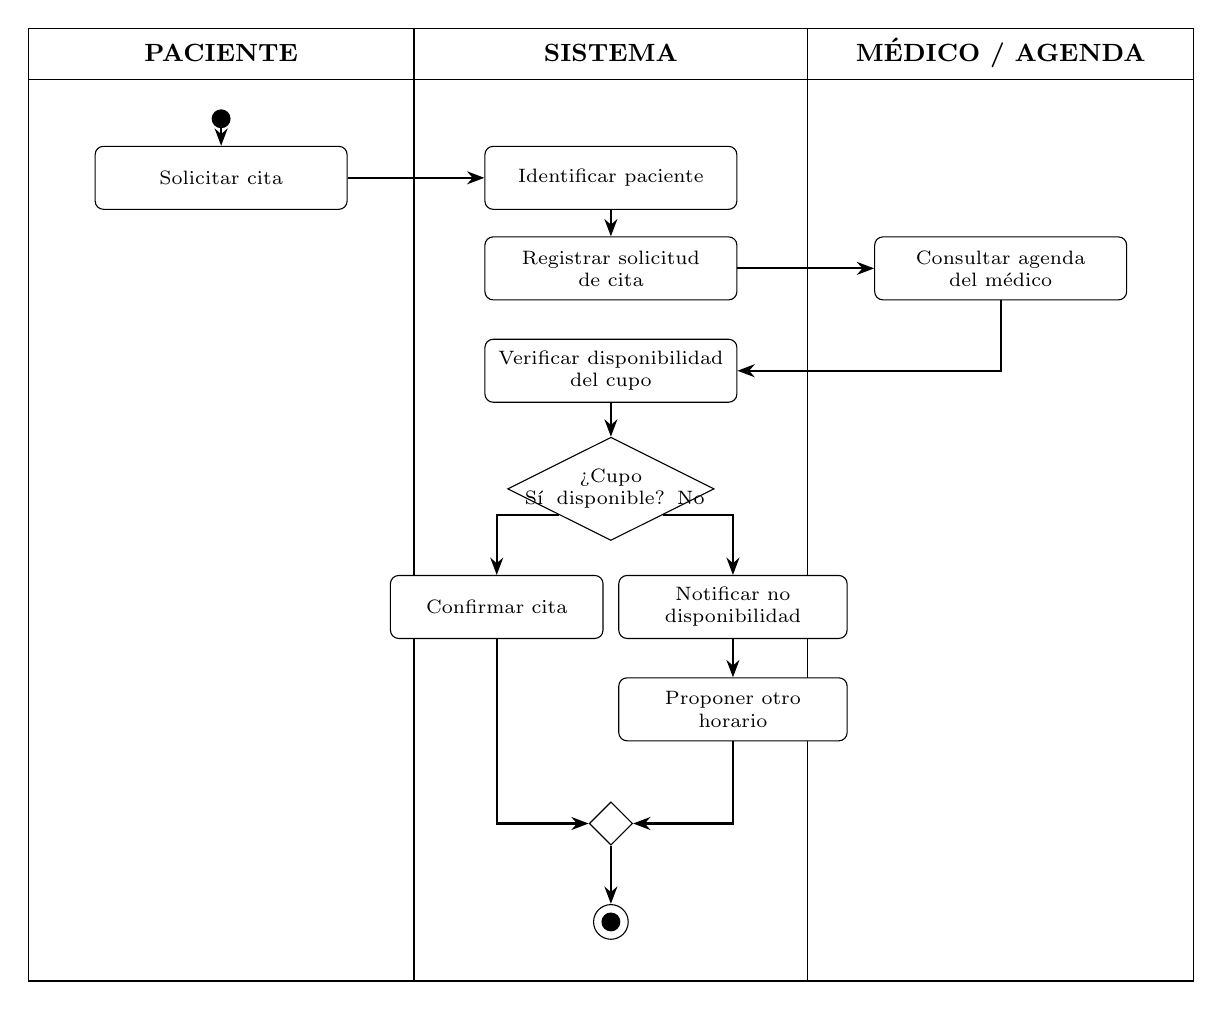
\begin{tikzpicture}[x=1cm,y=1cm]
% Carriles
\draw (-7.4,7.0) rectangle (7.4,-5.1);
\draw (-2.5,7.0) -- (-2.5,-5.1);
\draw (2.5,7.0) -- (2.5,-5.1);
\draw (-7.4,6.35) -- (7.4,6.35);
\node[font=\small\bfseries] at (-4.95,6.68) {PACIENTE};
\node[font=\small\bfseries] at (0,6.68) {SISTEMA};
\node[font=\small\bfseries] at (4.95,6.68) {M\'EDICO / AGENDA};

\fill (-4.95,5.85) circle (0.12);
\node[activity] (sol) at (-4.95,5.1) {Solicitar cita};
\node[activity] (id) at (0,5.1) {Identificar paciente};
\node[activity] (reg) at (0,3.95) {Registrar solicitud\\de cita};
\node[activity] (agenda) at (4.95,3.95) {Consultar agenda\\del m\'edico};
\node[activity] (ver) at (0,2.65) {Verificar disponibilidad\\del cupo};
\node[decision] (dec) at (0,1.15) {\textquestiondown Cupo\\disponible?};
\node[activity,minimum width=2.7cm] (conf) at (-1.45,-0.35) {Confirmar cita};
\node[activity,minimum width=2.9cm] (notif) at (1.55,-0.35) {Notificar no\\disponibilidad};
\node[activity,minimum width=2.9cm] (prop) at (1.55,-1.65) {Proponer otro\\horario};
\node[decision,aspect=1.2,minimum size=0.55cm,inner sep=0pt] (merge) at (0,-3.1) {};
\draw (0,-4.35) circle (0.22); \fill (0,-4.35) circle (0.12);

\draw[flow] (-4.95,5.73) -- (sol.north);
\draw[flow] (sol.east) -- (id.west);
\draw[flow] (id.south) -- (reg.north);
\draw[flow] (reg.east) -- (agenda.west);
\draw[flow] (agenda.south) |- (ver.east);
\draw[flow] (ver.south) -- (dec.north);
\draw[flow] (dec.south west) -| node[font=\scriptsize,above,pos=.2]{S\'i} (conf.north);
\draw[flow] (dec.south east) -| node[font=\scriptsize,above,pos=.2]{No} (notif.north);
\draw[flow] (notif.south) -- (prop.north);
\draw[flow] (conf.south) |- (merge.west);
\draw[flow] (prop.south) |- (merge.east);
\draw[flow] (merge.south) -- (0,-4.12);
\end{tikzpicture}
\captionof{figure}{Diagrama de actividades UML del proceso ``Agendar cita''.}
\end{center}

% ---------------------------------------------------------------------
% P3
% ---------------------------------------------------------------------
\begin{tarea}{P3. Modelo de comportamiento --- M\'aquina de estados UML \hfill (8 pts)}
Elabore la \textbf{m\'aquina de estados UML} del ciclo de vida de una \textsf{Cita} (p.\,ej. \textsf{Solicitada}, \textsf{Confirmada}, \textsf{Atendida}, \textsf{Cancelada}, \textsf{No asistida}). Etiquete cada \textbf{transici\'on} con su \textbf{evento}, incluya al menos una \textbf{condici\'on de guarda} y marque el estado final de aceptaci\'on. Se valora el uso de un superestado (statechart) para factorizar la transici\'on \emph{cancelar}.
\end{tarea}

\subsection*{Respuesta P3}
\begin{center}
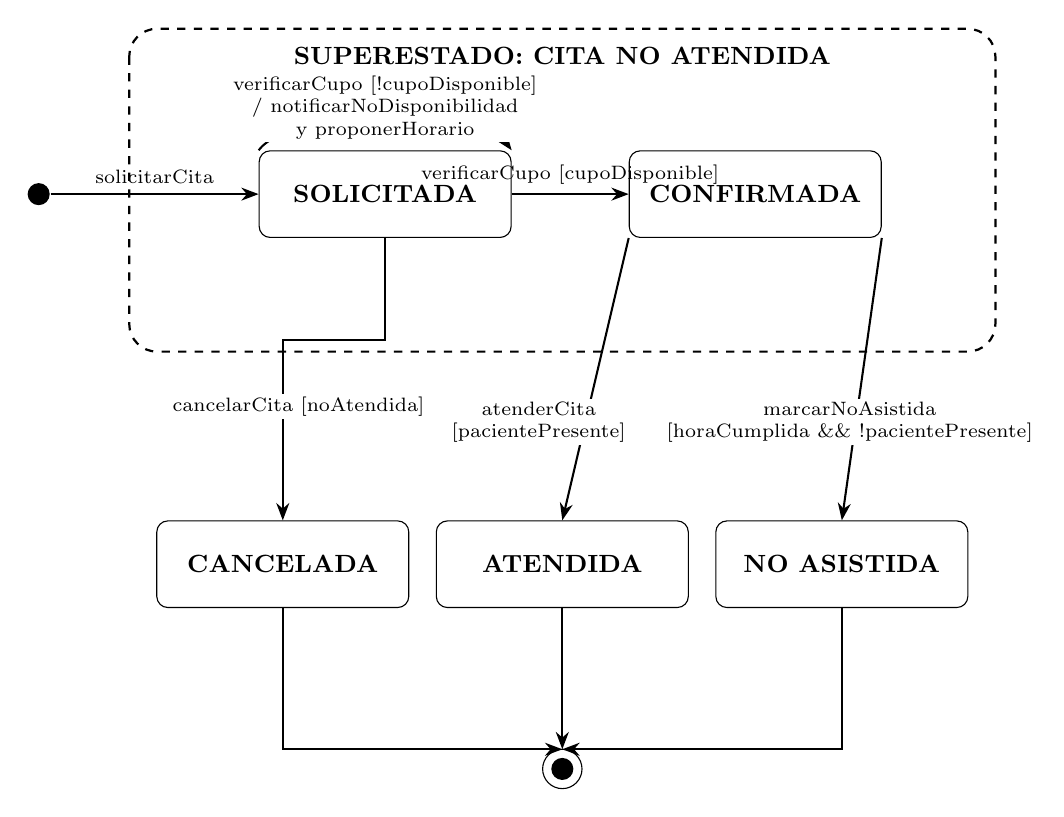
\begin{tikzpicture}[x=1cm,y=1cm]
% Superestado
\draw[dashed,rounded corners=10pt,line width=.8pt] (-5.5,4.65) rectangle (5.5,0.55);
\node[font=\small\bfseries] at (0,4.30) {SUPERESTADO: CITA NO ATENDIDA};

\node[state] (solic) at (-2.25,2.55) {SOLICITADA};
\node[state] (confir) at (2.45,2.55) {CONFIRMADA};
\node[state] (canc) at (-3.55,-2.15) {CANCELADA};
\node[state] (aten) at (0,-2.15) {ATENDIDA};
\node[state] (noas) at (3.55,-2.15) {NO ASISTIDA};
\fill (-6.65,2.55) circle (.14);
\draw (0,-4.75) circle (.25); \fill (0,-4.75) circle (.14);

\draw[flow] (-6.5,2.55) -- node[font=\scriptsize,above]{solicitarCita} (solic.west);
\draw[flow] (solic.east) -- node[font=\scriptsize,above]{verificarCupo [cupoDisponible]} (confir.west);

\draw[flow] (solic.north west) .. controls (-3.45,3.65) and (-1.05,3.65) .. (solic.north east);
\node[font=\scriptsize,align=center,fill=white,inner sep=1pt] at (-2.25,3.65)
{verificarCupo [!cupoDisponible]\\/ notificarNoDisponibilidad\\y proponerHorario};

\draw[flow] (solic.south) -- ++(0,-1.30) -| (canc.north);
\node[font=\scriptsize,fill=white,inner sep=1pt] at (-3.35,-0.15) {cancelarCita [noAtendida]};

\draw[flow] (confir.south west) -- (aten.north);
\node[font=\scriptsize,align=center,fill=white,inner sep=1pt] at (-0.30,-0.35)
{atenderCita\\{[pacientePresente]}};

\draw[flow] (confir.south east) -- (noas.north);
\node[font=\scriptsize,align=center,fill=white,inner sep=1pt] at (3.65,-0.35)
{marcarNoAsistida\\{[horaCumplida \&\& !pacientePresente]}};

\draw[flow] (canc.south) |- (0,-4.50);
\draw[flow] (aten.south) -- (0,-4.50);
\draw[flow] (noas.south) |- (0,-4.50);
\end{tikzpicture}
\captionof{figure}{M\'aquina de estados UML del ciclo de vida de una cita.}
\end{center}

% ---------------------------------------------------------------------
% P4
% ---------------------------------------------------------------------
\begin{tarea}{P4. Consistencia entre las tres perspectivas \hfill (7 pts)}
Elabore una \textbf{tabla de verificaci\'on cruzada} que relacione cada \textbf{evento} de P3 con la \textbf{funci\'on/acci\'on} de P2 que lo realiza y con la \textbf{entidad o atributo} de P1 que modifica. \textbf{Detecte al menos una inconsistencia} entre los modelos (evento sin funci\'on, entidad sin clase, etc.), \textbf{documente} el defecto y \textbf{corrija} el modelo afectado.
\end{tarea}

\subsection*{Respuesta P4}
\begin{center}
\scriptsize
\begin{tabularx}{\linewidth}{@{}L{3.7cm} X X@{}}
\toprule
\hd{Evento de P3} & \hd{Acci\'on o funci\'on de P2} & \hd{Entidad / atributo de P1 relacionado}\\
\midrule
\texttt{solicitarCita} & Solicitar cita / Registrar solicitud de cita & \texttt{Cita.idCita}, \texttt{Cita.fechaHora}, \texttt{Cita.estado}\\
\rowcolor{rowgray}
\texttt{verificarCupo} & Verificar disponibilidad del cupo / Consultar agenda del m\'edico & \texttt{Cupo.disponibilidad}\\
\texttt{confirmarCita} & Confirmar cita & \texttt{Cita.estado}, asociaci\'on \texttt{Cita-Cupo}\\
\rowcolor{rowgray}
\texttt{notificarNoDisponibilidad} & Notificar no disponibilidad & No modifica atributos; consulta \texttt{Cupo.disponibilidad}\\
\texttt{proponerHorario} & Proponer otro horario & \texttt{Cupo.fechaHora}\\
\rowcolor{rowgray}
\texttt{cancelarCita} & \textbf{No representado en P2} & \texttt{Cita.estado}\\
\texttt{atenderCita} & \textbf{No representado en P2} & \texttt{Cita.estado}\\
\rowcolor{rowgray}
\texttt{marcarNoAsistida} & \textbf{No representado en P2} & \texttt{Cita.estado}\\
\bottomrule
\end{tabularx}
\end{center}

\subsubsection*{Inconsistencia detectada --- INC-01}
En la m\'aquina de estados P3 aparecen los eventos \texttt{cancelarCita}, \texttt{atenderCita} y \texttt{marcarNoAsistida}, pero en el diagrama de actividades P2 no est\'an representadas las acciones correspondientes. Por lo tanto, existe una inconsistencia entre el modelo funcional y el modelo de comportamiento.

\subsubsection*{Correcci\'on del modelo afectado}
\textbf{Modelo corregido:} P2 --- Diagrama de actividades.\\
\textbf{Correcci\'on realizada:} se incorporan las acciones \textit{Esperar fecha de la cita}, \textit{Cancelar cita}, \textit{Atender cita} y \textit{Marcar cita no asistida}, junto con las decisiones \textit{\textquestiondown Cita cancelada?} y \textit{\textquestiondown Paciente se presenta?}.

\begin{center}
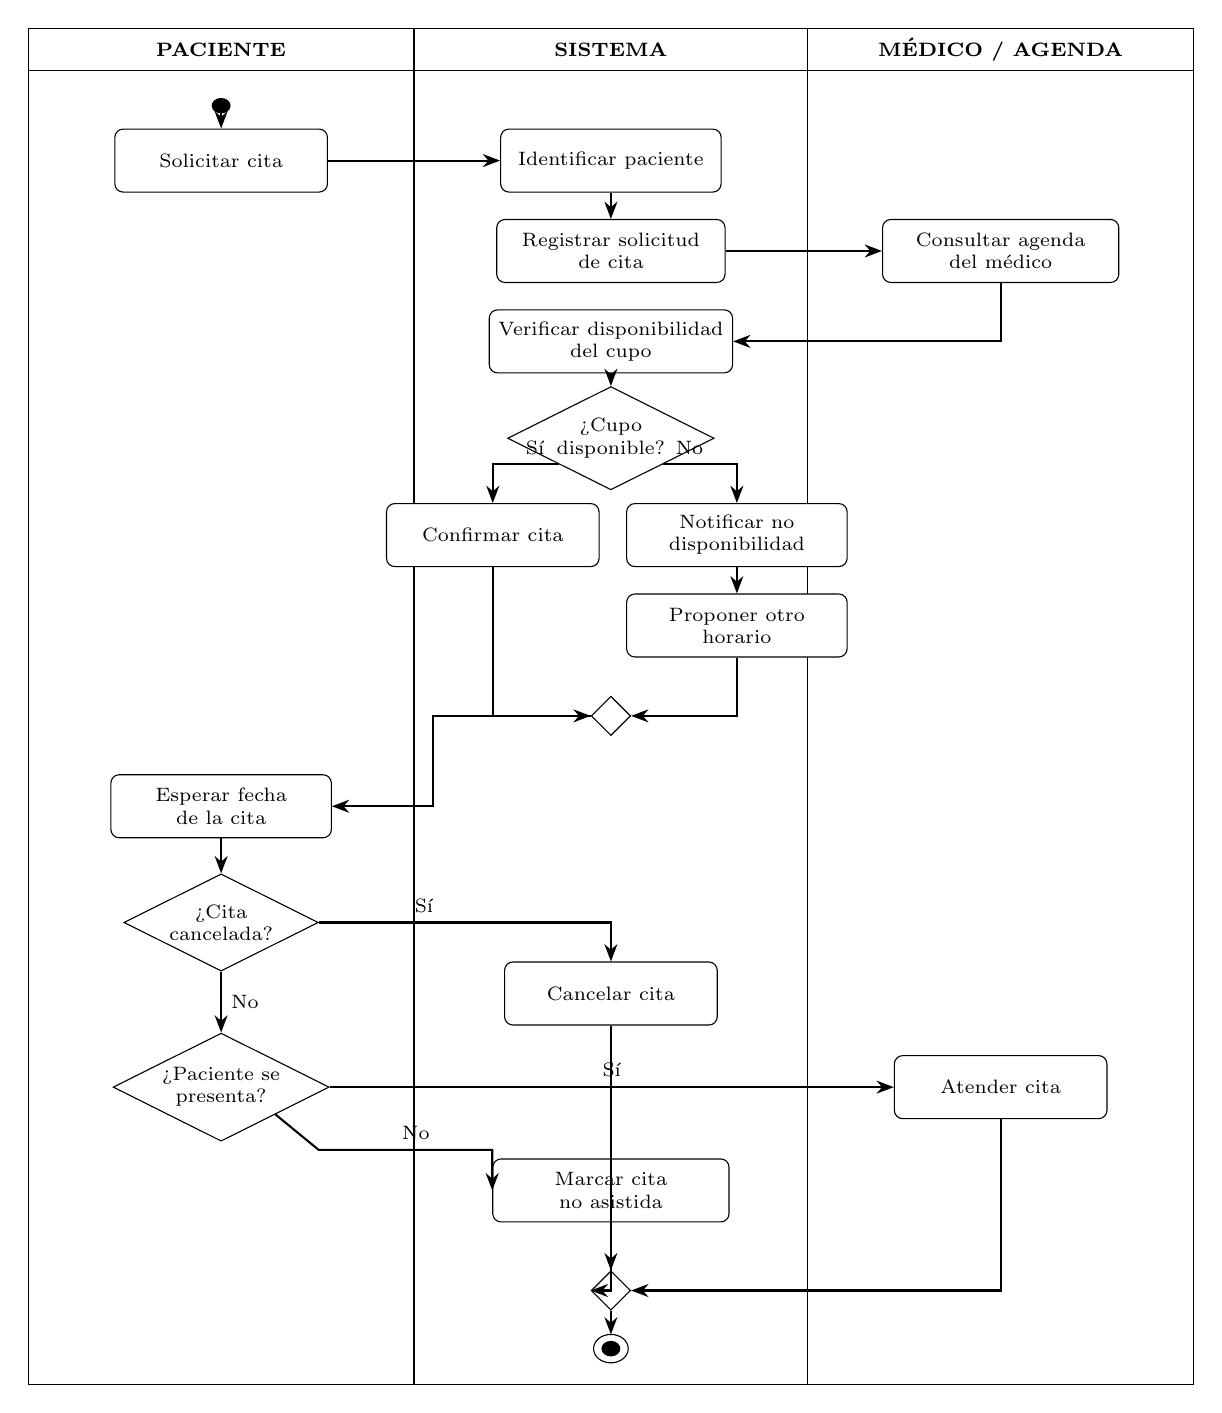
\begin{tikzpicture}[x=1cm,y=.82cm]
% Carriles P2 corregido
\draw (-7.4,10.6) rectangle (7.4,-10.4);
\draw (-2.5,10.6) -- (-2.5,-10.4);
\draw (2.5,10.6) -- (2.5,-10.4);
\draw (-7.4,9.95) -- (7.4,9.95);
\node[font=\scriptsize\bfseries] at (-4.95,10.27) {PACIENTE};
\node[font=\scriptsize\bfseries] at (0,10.27) {SISTEMA};
\node[font=\scriptsize\bfseries] at (4.95,10.27) {M\'EDICO / AGENDA};

\fill (-4.95,9.4) circle (.12);
\node[activity,minimum width=2.7cm] (s2) at (-4.95,8.55) {Solicitar cita};
\node[activity,minimum width=2.8cm] (i2) at (0,8.55) {Identificar paciente};
\node[activity,minimum width=2.9cm] (r2) at (0,7.15) {Registrar solicitud\\de cita};
\node[activity,minimum width=3.0cm] (a2) at (4.95,7.15) {Consultar agenda\\del m\'edico};
\node[activity,minimum width=3.0cm] (v2) at (0,5.75) {Verificar disponibilidad\\del cupo};
\node[decision] (d2) at (0,4.25) {\textquestiondown Cupo\\disponible?};
\node[activity,minimum width=2.7cm] (c2) at (-1.5,2.75) {Confirmar cita};
\node[activity,minimum width=2.8cm] (n2) at (1.6,2.75) {Notificar no\\disponibilidad};
\node[activity,minimum width=2.8cm] (p2) at (1.6,1.35) {Proponer otro\\horario};
\node[decision,aspect=1.2,minimum size=.5cm,inner sep=0pt] (m2) at (0,-.05) {};
\node[activity,minimum width=2.8cm] (wait) at (-4.95,-1.45) {Esperar fecha\\de la cita};
\node[decision] (cancelq) at (-4.95,-3.25) {\textquestiondown Cita\\cancelada?};
\node[activity,minimum width=2.7cm] (cancelact) at (0,-4.35) {Cancelar cita};
\node[decision] (presentq) at (-4.95,-5.80) {\textquestiondown Paciente se\\presenta?};
\node[activity,minimum width=2.7cm] (attend) at (4.95,-5.80) {Atender cita};
\node[activity,minimum width=3.0cm] (noassist) at (0,-7.40) {Marcar cita\\no asistida};
\node[decision,aspect=1.2,minimum size=.5cm,inner sep=0pt] (mfinal) at (0,-8.95) {};
\draw (0,-9.85) circle (.22); \fill (0,-9.85) circle (.12);

\draw[flow] (-4.95,9.28) -- (s2.north);
\draw[flow] (s2.east) -- (i2.west);
\draw[flow] (i2.south) -- (r2.north);
\draw[flow] (r2.east) -- (a2.west);
\draw[flow] (a2.south) |- (v2.east);
\draw[flow] (v2.south) -- (d2.north);
\draw[flow] (d2.south west) -| node[font=\scriptsize,above,pos=.18]{S\'i} (c2.north);
\draw[flow] (d2.south east) -| node[font=\scriptsize,above,pos=.18]{No} (n2.north);
\draw[flow] (n2.south) -- (p2.north);
\draw[flow] (c2.south) |- (m2.west);
\draw[flow] (p2.south) |- (m2.east);
\draw[flow] (m2.west) -- ++(-2.0,0) |- (wait.east);
\draw[flow] (wait.south) -- (cancelq.north);
\draw[flow] (cancelq.east) -| node[font=\scriptsize,above,pos=.18]{S\'i} (cancelact.north);
\draw[flow] (cancelq.south) -- node[font=\scriptsize,right]{No} (presentq.north);
\draw[flow] (presentq.east) -- node[font=\scriptsize,above]{S\'i} (attend.west);
\draw[flow] (presentq.south east) -- ++(.55,-.55) -| node[font=\scriptsize,above,pos=.28]{No} (noassist.west);
\draw[flow] (cancelact.south) |- (mfinal.west);
\draw[flow] (noassist.south) -- (mfinal.north);
\draw[flow] (attend.south) |- (mfinal.east);
\draw[flow] (mfinal.south) -- (0,-9.63);
\end{tikzpicture}
\captionof{figure}{P2 corregido tras documentar la inconsistencia INC-01.}
\end{center}

Al realizar la verificaci\'on cruzada entre P1, P2 y P3, se detect\'o la inconsistencia \textbf{INC-01}, debido a que en la m\'aquina de estados se definieron los eventos \texttt{cancelarCita}, \texttt{atenderCita} y \texttt{marcarNoAsistida}, pero dichas acciones no estaban representadas en el diagrama de actividades. Para corregir esta inconsistencia, se actualiz\'o el modelo funcional incorporando las acciones \textit{Cancelar cita}, \textit{Atender cita} y \textit{Marcar cita no asistida}, as\'i como las decisiones \textit{\textquestiondown Cita cancelada?} y \textit{\textquestiondown Paciente se presenta?}. Luego de la correcci\'on, los tres modelos mantienen coherencia entre eventos, funciones y entidades.

% ---------------------------------------------------------------------
% P5
% ---------------------------------------------------------------------
\begin{tarea}{P5. Especificaci\'on de requisitos con esquema de atributos \hfill (10 pts)}
Redacte \textbf{4 requisitos}: \textbf{2 funcionales} y \textbf{2 no funcionales}. Cada requisito no funcional debe \textbf{nombrar una caracter\'istica de \textit{ISO/IEC} 25010:2023} (p.\,ej. Eficiencia de desempe\~no, Seguridad), fijar una \textbf{m\'etrica} y un \textbf{umbral} (p.\,ej. ``agendar la cita en $<$ 3 s''). Para cada requisito complete un \textbf{esquema de atributos}: identificador, prioridad, estado, fuente, estabilidad, versi\'on y m\'etodo de verificaci\'on.
\end{tarea}

\subsection*{Respuesta P5}
\begin{reqbox}{RF-01 --- Registrar cita}
\small
\begin{tabularx}{\linewidth}{@{}L{3.4cm} X@{}}
\textbf{Identificador} & RF-01\\
\textbf{Tipo} & Funcional\\
\textbf{Nombre} & Registrar cita\\
\textbf{Requisito} & El sistema deber\'a registrar una cita solicitada por un paciente, asoci\'andola con un m\'edico y un cupo de su agenda.\\
\textbf{Prioridad} & Alta\\
\textbf{Estado} & En revisi\'on\\
\textbf{Fuente} & Caso pr\'actico: Sistema de Reserva de Citas M\'edicas\\
\textbf{Estabilidad} & Alta\\
\textbf{Versi\'on} & 1.0\\
\textbf{M\'etodo de verificaci\'on} & Prueba de aceptaci\'on PA-01\\
\end{tabularx}
\end{reqbox}

\begin{reqbox}{RF-02 --- Verificar disponibilidad del cupo}
\small
\begin{tabularx}{\linewidth}{@{}L{3.4cm} X@{}}
\textbf{Identificador} & RF-02\\
\textbf{Tipo} & Funcional\\
\textbf{Nombre} & Verificar disponibilidad del cupo\\
\textbf{Requisito} & El sistema deber\'a verificar la disponibilidad del cupo seleccionado antes de confirmar una cita.\\
\textbf{Prioridad} & Alta\\
\textbf{Estado} & En revisi\'on\\
\textbf{Fuente} & Caso pr\'actico: disponibilidad de cupos\\
\textbf{Estabilidad} & Alta\\
\textbf{Versi\'on} & 1.0\\
\textbf{M\'etodo de verificaci\'on} & Prueba de aceptaci\'on PA-02\\
\end{tabularx}
\end{reqbox}

\begin{reqbox}{RNF-01 --- Tiempo de respuesta}
\small
\begin{tabularx}{\linewidth}{@{}L{3.4cm} X@{}}
\textbf{Identificador} & RNF-01\\
\textbf{Tipo} & No funcional\\
\textbf{Nombre} & Tiempo de registro de la cita\\
\textbf{Caracter\'istica ISO/IEC 25010:2023} & Eficiencia de desempe\~no\\
\textbf{Requisito} & Desde que el paciente solicita agendar una cita hasta que el sistema presenta el resultado de la solicitud, el tiempo de respuesta deber\'a ser inferior a 3 segundos.\\
\textbf{M\'etrica} & Tiempo de respuesta\\
\textbf{Umbral} & $<$ 3 segundos\\
\textbf{Prioridad} & Alta\\
\textbf{Estado} & En revisi\'on\\
\textbf{Fuente} & Caso pr\'actico: registrar la cita con rapidez\\
\textbf{Estabilidad} & Alta\\
\textbf{Versi\'on} & 1.0\\
\textbf{M\'etodo de verificaci\'on} & Prueba de rendimiento PA-03\\
\end{tabularx}
\end{reqbox}

\begin{reqbox}{RNF-02 --- Protecci\'on de datos personales}
\small
\begin{tabularx}{\linewidth}{@{}L{3.4cm} X@{}}
\textbf{Identificador} & RNF-02\\
\textbf{Tipo} & No funcional\\
\textbf{Nombre} & Protecci\'on de datos personales\\
\textbf{Caracter\'istica ISO/IEC 25010:2023} & Seguridad\\
\textbf{Requisito} & El sistema deber\'a impedir que usuarios no autorizados visualicen la c\'edula, nombre y correo de los pacientes.\\
\textbf{M\'etrica} & Porcentaje de accesos no autorizados que permiten visualizar datos personales\\
\textbf{Umbral} & 0\%\\
\textbf{Prioridad} & Alta\\
\textbf{Estado} & En revisi\'on\\
\textbf{Fuente} & Caso pr\'actico: protecci\'on de datos personales del paciente\\
\textbf{Estabilidad} & Alta\\
\textbf{Versi\'on} & 1.0\\
\textbf{M\'etodo de verificaci\'on} & Prueba de seguridad PA-04\\
\end{tabularx}
\end{reqbox}

% ---------------------------------------------------------------------
% P6
% ---------------------------------------------------------------------
\begin{tarea}{P6. Priorizaci\'on MoSCoW \hfill (5 pts)}
Clasifique los 4 requisitos de P5 en las categor\'ias \textbf{MoSCoW} (\textit{Must / Should / Could / Won't have this time}) y \textbf{justifique} brevemente cada asignaci\'on en funci\'on del valor y la viabilidad. Al menos un requisito debe ser \textit{Must have}.
\end{tarea}

\subsection*{Respuesta P6}
\begin{center}
\small
\begin{tabularx}{\linewidth}{@{}L{3.2cm} C{2.3cm} X@{}}
\toprule
\hd{Requisito} & \hd{Prioridad MoSCoW} & \hd{Justificaci\'on}\\
\midrule
RF-01 --- Registrar cita & Must Have & Es indispensable para el funcionamiento del sistema, ya que permite registrar las citas solicitadas por los pacientes.\\
\rowcolor{rowgray}
RF-02 --- Verificar disponibilidad del cupo & Must Have & Es necesario para evitar la confirmaci\'on de citas en horarios que no tengan disponibilidad.\\
RNF-01 --- Tiempo de respuesta & Should Have & Es importante que el registro de una cita se realice en menos de 3 segundos para ofrecer un servicio r\'apido, aunque el sistema podr\'ia continuar funcionando si temporalmente supera ese tiempo.\\
\rowcolor{rowgray}
RNF-02 --- Protecci\'on de datos personales & Must Have & Es indispensable proteger la c\'edula, nombre y correo de los pacientes e impedir el acceso de usuarios no autorizados.\\
\bottomrule
\end{tabularx}
\end{center}

\textbf{Must Have:} RF-01, RF-02 y RNF-02.\\
\textbf{Should Have:} RNF-01.

% ---------------------------------------------------------------------
% P7
% ---------------------------------------------------------------------
\begin{tarea}{P7. Validaci\'on por inspecci\'on (lista de comprobaci\'on 29148) \hfill (8 pts)}
Aplique a los requisitos de P5 una \textbf{lista de comprobaci\'on} derivada de las propiedades de \textit{ISO/IEC/IEEE} 29148 (no ambiguo, completo, singular, verificable, factible). \textbf{Registre los defectos detectados sin corregirlos en el momento} (separar identificaci\'on de correcci\'on) y, en un segundo paso, presente el \textbf{retrabajo} con los requisitos corregidos.
\end{tarea}

\subsection*{Respuesta P7}
\subsubsection*{1. Inspecci\'on de requisitos}
\begin{center}
\scriptsize
\begin{tabularx}{\linewidth}{@{}L{2.1cm} C{1.35cm} C{1.2cm} C{1.15cm} C{1.35cm} C{1.15cm} X@{}}
\toprule
\hd{Requisito} & \hd{No ambiguo} & \hd{Completo} & \hd{Singular} & \hd{Verificable} & \hd{Factible} & \hd{Defecto}\\
\midrule
RF-01 Registrar cita & S\'i & S\'i & S\'i & S\'i & S\'i & Ninguno\\
\rowcolor{rowgray}
RF-02 Verificar disponibilidad del cupo & S\'i & S\'i & S\'i & S\'i & S\'i & Ninguno\\
RNF-01 Tiempo de respuesta & \textbf{No} & S\'i & S\'i & S\'i & S\'i & ``Resultado de la solicitud'' no especifica claramente cu\'al resultado\\
\rowcolor{rowgray}
RNF-02 Protecci\'on de datos personales & \textbf{No} & S\'i & S\'i & S\'i & S\'i & ``Usuario no autorizado'' no define con precisi\'on qui\'en carece de autorizaci\'on\\
\bottomrule
\end{tabularx}
\end{center}

\subsubsection*{2. Registro de defectos --- antes de corregir}
\textbf{DEF-01}\\
\textbf{Requisito:} RNF-01.\\
\textbf{Propiedad afectada:} No ambiguo.\\
La expresi\'on ``resultado de la solicitud'' puede interpretarse de diferentes maneras, ya que no especifica si el resultado corresponde a la confirmaci\'on de la cita o a la notificaci\'on de no disponibilidad.

\textbf{DEF-02}\\
\textbf{Requisito:} RNF-02.\\
\textbf{Propiedad afectada:} No ambiguo.\\
La expresi\'on ``usuarios no autorizados'' no especifica claramente qu\'e condici\'on determina que un usuario no posea autorizaci\'on para consultar los datos personales del paciente.

\subsubsection*{3. Retrabajo de requisitos}
\textbf{RNF-01 corregido --- Versi\'on 1.1}\\
Desde que el paciente solicita agendar una cita hasta que el sistema muestra la confirmaci\'on de la cita o la notificaci\'on de no disponibilidad del cupo, el tiempo de respuesta deber\'a ser inferior a 3 segundos.\\
\textbf{M\'etrica:} Tiempo de respuesta.\\
\textbf{Umbral:} $<$ 3 segundos.

\textbf{RNF-02 corregido --- Versi\'on 1.1}\\
El sistema deber\'a impedir que los usuarios que no posean permisos de consulta de datos personales visualicen la c\'edula, nombre y correo de los pacientes.\\
\textbf{M\'etrica:} Porcentaje de accesos sin permiso que permiten visualizar datos personales.\\
\textbf{Umbral:} 0\%.

\subsubsection*{4. Reinspecci\'on despu\'es del retrabajo}
\begin{center}
\small
\begin{tabularx}{\linewidth}{@{}L{3cm} C{2cm} C{1.7cm} C{1.7cm} C{2cm} C{1.7cm}@{}}
\toprule
\hd{Requisito} & \hd{No ambiguo} & \hd{Completo} & \hd{Singular} & \hd{Verificable} & \hd{Factible}\\
\midrule
RF-01 v1.0 & S\'i & S\'i & S\'i & S\'i & S\'i\\
\rowcolor{rowgray}
RF-02 v1.0 & S\'i & S\'i & S\'i & S\'i & S\'i\\
RNF-01 v1.1 & S\'i & S\'i & S\'i & S\'i & S\'i\\
\rowcolor{rowgray}
RNF-02 v1.1 & S\'i & S\'i & S\'i & S\'i & S\'i\\
\bottomrule
\end{tabularx}
\end{center}

Despu\'es del retrabajo de los defectos \textbf{DEF-01} y \textbf{DEF-02}, los cuatro requisitos cumplen con las propiedades de calidad evaluadas: no ambiguo, completo, singular, verificable y factible.

% ---------------------------------------------------------------------
% P8, P9, P10: se conservan tal como aparecen en el instrumento, sin resolver.
% ---------------------------------------------------------------------
\begin{tarea}{P8. Pruebas de aceptaci\'on trazadas \hfill (6 pts)}
Defina \textbf{una prueba de aceptaci\'on por requisito} (4 en total), indicando su \textbf{tipo} (funcional, no funcional o regresi\'on), sus \textbf{entradas}, el \textbf{criterio de \'exito} y el \textbf{requisito al que traza}. Cada prueba debe enlazar expl\'icitamente con al menos un requisito de P5.
\end{tarea}

\begin{tarea}{P9. Matriz de trazabilidad \hfill (6 pts)}
Construya la \textbf{matriz de trazabilidad} que cruce los requisitos con: su \textbf{fuente} (traza hacia atr\'as) y sus \textbf{modelos y pruebas de aceptaci\'on} (traza hacia adelante). Marque tambi\'en al menos una dependencia \textbf{horizontal} entre requisitos e \textbf{identifique} cualquier requisito hu\'erfano (sin prueba o sin modelo asociado).
\end{tarea}

\begin{tarea}{P10. Gesti\'on del cambio y l\'inea base \hfill (4 pts)}
Simule \textbf{una solicitud de cambio} sobre un requisito: reg\'istrela, \textbf{analice su impacto} usando la matriz de P9, indique la \textbf{decisi\'on del CCB} (aprobada/rechazada/diferida) y \textbf{actualice la versi\'on} del requisito. Finalmente, declare una \textbf{l\'inea base}: liste la \textbf{configuraci\'on} (versiones coherentes de ERS, modelos, matriz y pruebas) que se congela.
\end{tarea}

% =====================================================================
\section{R\'ubrica de evaluaci\'on}

La calificaci\'on total es de \textbf{100 puntos}, distribuidos en \textbf{30\%} para el cuestionario rendido en el LMS (SGA) y \textbf{70\%} para el desarrollo de la prueba pr\'actica. Los \textbf{criterios de piso} de la Secci\'on~1 se aplican \emph{antes} de sumar puntos: si alguno se incumple, la calificaci\'on final es \textbf{CERO}, con independencia de los puntos logrados en cada criterio.

\begin{concepto}{Escala de niveles de logro (se aplica a cada criterio de la prueba pr\'actica)}
\textbf{Logrado (100\% del peso):} el producto cumple \'integramente lo solicitado, es correcto y consistente. \quad \textbf{Parcial (60\%):} cumple lo esencial pero con omisiones o errores menores. \quad \textbf{Insuficiente (30\%):} entrega incompleta o con errores conceptuales relevantes. \quad \textbf{No entregado (0\%):} ausente o no evaluable.
\end{concepto}

\begin{table}[htbp]
  \centering
  \caption{Componente 1 --- Cuestionario en el LMS (SGA). Peso: 30 puntos.}
  \small
  \begin{tabularx}{\linewidth}{@{}L{4.6cm} C{1.6cm} X@{}}
    \toprule
    \hd{Criterio} & \hd{Peso} & \hd{Evidencia requerida}\\
    \midrule
    Nota obtenida en el cuestionario del SGA & 20 pts & Puntaje autocalificado por el LMS, proporcional al porcentaje de aciertos.\\
    \rowcolor{rowgray}
    Captura del \emph{resumen} del cuestionario en la car\'atula & 5 pts & Imagen legible del resumen de resultados incrustada en la portada del PDF.\\
    Captura de la \emph{evaluaci\'on} (intento) en la car\'atula & 5 pts & Imagen legible del intento/evaluaci\'on incrustada en la portada del PDF.\\
    \bottomrule
  \end{tabularx}
\end{table}

\begin{landscape}
\begin{table}[htbp]
  \centering
  \caption{Componente 2 --- Desarrollo de la prueba pr\'actica. Peso: 70 puntos. (Logrado 100\% / Parcial 60\% / Insuficiente 30\% / No entregado 0\% del peso indicado.)}
  \scriptsize
  \renewcommand{\arraystretch}{1.2}
  \begin{tabularx}{\linewidth}{@{}L{3.0cm} C{0.9cm} X X X@{}}
    \toprule
    \hd{Criterio (tarea)} & \hd{Peso} & \hd{Logrado (100\%)} & \hd{Parcial (60\%)} & \hd{Insuficiente (30\%)}\\
    \midrule
    P1. Diagrama de clases UML & 8 & Clases, atributos tipados, operaciones y multiplicidades correctas y coherentes con el caso. & Faltan operaciones o alguna multiplicidad; estructura b\'asica correcta. & Clases incompletas o sin multiplicidades; errores de modelado.\\
    \rowcolor{rowgray}
    P2. Diagrama de actividades UML & 8 & Decisi\'on de \textit{cupo}, ambos caminos, convergencia y nodo final bien modelados. & Flujo correcto pero sin decisi\'on o sin convergencia expl\'icita. & Secuencia lineal sin l\'ogica de control del caso.\\
    P3. M\'aquina de estados UML & 8 & Estados, eventos, guarda y estado final; superestado bien usado. & Estados y eventos correctos, sin guarda o sin estado final. & Estados incompletos o transiciones sin evento.\\
    \rowcolor{rowgray}
    P4. Consistencia entre perspectivas & 7 & Tabla cruzada completa; inconsistencia detectada, documentada y corregida. & Tabla parcial o inconsistencia detectada pero no corregida. & Tabla ausente o sin an\'alisis de correspondencia.\\
    P5. Requisitos con esquema de atributos & 10 & 4 requisitos (2 F, 2 NF) con caracter\'istica 25010, m\'etrica, umbral y atributos completos. & Requisitos correctos con atributos incompletos o sin umbral. & Requisitos ambiguos o sin esquema de atributos.\\
    \rowcolor{rowgray}
    P6. Priorizaci\'on MoSCoW & 5 & Cuatro requisitos clasificados y justificados; al menos un \textit{Must}. & Clasificaci\'on correcta con justificaci\'on d\'ebil. & Clasificaci\'on sin justificar o mal aplicada.\\
    P7. Inspecci\'on 29148 (defectos + retrabajo) & 8 & Checklist aplicada; defectos registrados sin corregir y retrabajo presentado. & Defectos detectados sin retrabajo, o correcci\'on mezclada con detecci\'on. & Sin checklist o sin evidencia de defectos.\\
    \rowcolor{rowgray}
    P8. Pruebas de aceptaci\'on trazadas & 6 & 4 pruebas con tipo, entradas, criterio de \'exito y traza al requisito. & Pruebas sin tipo o sin criterio de \'exito claro. & Pruebas sin traza a requisitos.\\
    P9. Matriz de trazabilidad & 6 & Trazas hacia atr\'as, adelante y horizontal; hu\'erfanos identificados. & Matriz parcial (solo un sentido de traza). & Matriz ausente o sin correspondencias reales.\\
    \rowcolor{rowgray}
    P10. Gesti\'on del cambio y l\'inea base & 4 & Solicitud, impacto, decisi\'on CCB, versi\'on y configuraci\'on/baseline declarada. & Cambio registrado sin impacto o sin baseline. & Sin proceso de cambio ni l\'inea base.\\
    \midrule
    \hg{Total del componente pr\'actico} & \hg{70} & \multicolumn{3}{c}{\cellcolor{lightgray}\small\color{darkblue} Suma de puntos logrados por nivel en cada criterio.}\\
    \bottomrule
  \end{tabularx}
\end{table}
\end{landscape}

\begin{table}[htbp]
  \centering
  \caption{Resumen de ponderaci\'on final.}
  \small
  \begin{tabularx}{\linewidth}{@{}X C{2.4cm} C{3.0cm}@{}}
    \toprule
    \hd{Componente} & \hd{Peso} & \hd{Condici\'on}\\
    \midrule
    Cuestionario en el LMS (SGA) + capturas en car\'atula & 30 pts & Sujeto a criterios de piso\\
    \rowcolor{rowgray}
    Desarrollo de la prueba pr\'actica (P1--P10) & 70 pts & Sujeto a criterios de piso\\
    \midrule
    \hg{Total} & \hg{100 pts} & \hg{CERO si se incumple un criterio de piso}\\
    \bottomrule
  \end{tabularx}
\end{table}

% =====================================================================
\section{Marco normativo de referencia}

Esta prueba operacionaliza las propiedades de calidad de la norma \textit{ISO/IEC/IEEE} 29148:2018 \citep{iso29148_2018} y el modelo de calidad de producto \textit{ISO/IEC} 25010:2023 \citep{iso25010_2023}, junto con las t\'ecnicas de validaci\'on y gesti\'on descritas por Pohl \citep{pohl_2010}, la inspecci\'on formal de Fagan \citep{fagan_1976} y las buenas pr\'acticas recogidas en la gu\'ia SWEBOK v4 \citep{swebok_v4_2024}. Las notaciones de modelado siguen la especificaci\'on \textit{OMG UML} 2.5.1 \citep{omg_uml_2017}.

\vspace{4pt}
\renewcommand{\refname}{Referencias}
\begin{thebibliography}{99}
\small
\bibitem{iso29148_2018} ISO/IEC/IEEE. (2018). \textit{ISO/IEC/IEEE 29148:2018 Systems and software engineering --- Life cycle processes --- Requirements engineering}. International Standard.
\bibitem{iso25010_2023} ISO/IEC. (2023). \textit{ISO/IEC 25010:2023 Systems and software engineering --- Systems and software Quality Requirements and Evaluation (SQuaRE) --- Product quality model}. International Standard.
\bibitem{omg_uml_2017} Object Management Group. (2017). \textit{Unified Modeling Language (OMG UML), Version 2.5.1}. OMG Standard, document formal/2017-12-05.
\bibitem{swebok_v4_2024} Washizaki, H. (Ed.). (2024). \textit{Guide to the Software Engineering Body of Knowledge (SWEBOK Guide), Version 4.0}. IEEE Computer Society.
\bibitem{pohl_2010} Pohl, K. (2010). \textit{Requirements Engineering: Fundamentals, Principles, and Techniques}. Springer.
\bibitem{fagan_1976} Fagan, M. E. (1976). Design and code inspections to reduce errors in program development. \textit{IBM Systems Journal}, 15(3), 182--211.
\end{thebibliography}

\end{document}
